\chapter{Realizace}
Po dohodě s vedoucím práce byl zvolen iterační vývoj aplikace. Za účelem postupného vyvíjený částí aplikace, tak aby bylo možné testovat aplikaci na letním semestru 2011/2012. V této kapitole popisuji jednotlivá zadání každé iterace. Jak jsem postupoval k vyřešení zadání a výstupy z jednotlivých iterací. Jednotlivé iterace byly prezentovány na konzultacích s vedoucím práce.

\section{První iterace}
\subsection{Zadání}
Tato iterace patřila k nejobsáhlejším ze všech iterací. Jedním z důvodů bylo  seznámení z novou technologii Ruby on Rails, s kterou jsem neměl zkušenost. První iterace měla za cíl navrhnout a vytvořit základní architekturu aplikace s napojením na KOSapi \cite{kosapi} a k tomu vytvořit funkční část aplikace pro plánování hospitací, tak abych mohl prezentovat funkčnost.

\subsection{Postup}
\subsubsection{Datová vrstva}
Protože aplikace využívá dva datové zdroje KOSapi viz. \ref{kosapi} a databázi aplikace, bylo potřeba nejdřív vyřešit jak se připojit ke KOSapi. V této části vycházím z prototypu aplikace pro správu hospitací. Kde využívá již naprogramovanou knihovnu z projektu VyVy \cite{vyvy}. Poté bylo potřeba vytvořil modely tak, aby umožnily komunikaci mezi KOSapi a databází aplikace. Při implementování knihovny do aplikace jsem musel vyřešit lokalizaci jazykových konstant v date získaných z API. Vyřešil jsem to rozšířením knihovny o podporu modul i18n\footnote{lokalizace softwaru pro různé jazyky a jejich místních zvyklostí}, který je součástí Rails.

\subsubsection{Autentizace}
Pro autentizaci, v této fázi vývoje, používám knihovnu authlogic, kterou jsem zprovoznil pomocí návodu \cite{authlogic}. Tuto knihovnu používám jen dočasně pro vývoj aplikace. Ve finální fázi bude nahrazen autentizační službou FELid viz. \ref{felid}, kterou lze zprovoznit jen na serveru, kde bude aplikace nasazena. 

\subsubsection{Autorizace}
Autentizace v hospitacích je jedena z kritických oblastí, kterou bylo potřeba vyřešit hned na začátku vývoje. V aplikaci potřebuji autentizovat uživatele podle role, tak i podle vztahu k hospitaci. Proto jsem hledal modul, který by dokázal nadefinovat pravidla autentizace. Knihovnu, kterou jsem použil, se jmenuje CanCan \cite{cancan} . Tato knihovna má velmi jednoduchý ale i přesto flexibilní zápis pravidel, která dokáží filtrovat jak podle zdroje tak i podle jednotlivých záznamů, dokáže filtrovat controllery tak i zdroje aplikace.  Veškerá pravidla jsou definována na jednom místě\footnote{model Ability} aplikace.

\begin{quote}
Příklad zapsaného pravidla pomocí CanCan v modelu Ability. Pravidlo slouží pro administrátora hospitací a umožní mu zobrazovat, vytvářet, upravovat a mazat ze zdroje Observation. Zároveň zakáže tyto operace pro záznamy, které nevytvořil.

\begin{verbatim}
def admin
    can :manage, Observation
    cannot :manage, Observation do |ob|
        !(ob.created_by==current_user)
    end
end
\end{verbatim} 
\end{quote}

\subsubsection{Role}
\label{sec:role}
Role pro jednotlivé uživatelé uchovávám v modelu Role. Kde jednotlivé role uživatele ukládám do bitové masky. Role v bitové masce jsou reprezentovány mocniny čísla 2 díky tomu lze skládat role pomocí bitové operace OR. V tabulce \ref{tab:role} je přehled rolí s číslem reprezentovaným bitovou masku role.

\begin{table}[h]
\begin{center}
\begin{tabular}{|l|c|}

\hline
\textbf{Role} & \textbf{Bitová maska} \\ \hline
Administrátor hospitací & 1 \\
Hospitující & 2 \\ 
Hospitovaný & 4 \\
Admin & 8 \\\hline

\end{tabular}
\caption{Reprezentace rolí v bitové masce}
\label{tab:role}
\end{center}
\end{table}

\subsubsection{Uživatelské prostředí}
Pro vytvoření uživatelského prostředí jsem použil již existující modul Bootstrap \cite{bootstrap}. Použil jsem tuto knihovnu abych si usnadnil implementaci uživatelského prostředí. Knihovna obsahuje kompletní CSS tak i Javascriptové moduly. Mezi další výhody patří licence ta je open-source a další výhodou je známé uživatelské prostředí používané v Twitteru.

Pro usnadnění implementace Bootstrap modulu do aplikace jsem využil další dva moduly pro aplikaci. První je modul SimpleForm \cite{simpleform}, slouží k vytváření formulářů. Základním cílem je nadefinovat rozvržení všech formulářů na jednom místě. Druhým modulem je WillPaginate \cite{willpaginate} pros stránkován dat.

\subsection{Výstup} 
Výstupem z první iterace vznikla část aplikace, která uměla plánovat hospitace a uměla získávat data z webové služby KOSapi.


\section{Druhá iterace}
\subsection{Zadání}
Zadáním druhé iterace bylo na-implementovat hodnotící formuláře hospitací. Požadavkem bylo možnost upravovat formuláře bez zásahu do kódu aplikace. Dalším cílem bylo potřeba vyřešit problém s KOSapi, který vznikl při přechodu na nový semestr. Stalo se to že služba neudržuje data instancí předmětů z minulých semestrů a tím nebylo možné získat všechny potřebné informace pro hospitace z minulých semestrů.

\subsection{Postup}
\subsubsection{Datová vrstva}
Problém se ztrátou dat byl velmi vážný, proto bylo potřeba tento problém rychle vyřešit abych mohl pokračovat ve vývoji. Musel jsem proto předělat datovou část. Rozšířil jsem databázi o entity z kapitoly \ref{sec:domeny_kosapi} tak, aby data z KOSapi byli uložené v databázi. Data je potřeba synchronizovat v databázi s KOSapi. O synchronizaci se stará \verb|rake|\footnote{rake je sada nástrojů používané pro vývoj a nasazení Rails aplikací} script stará se o přidává a aktualizaci záznamy. Synchronizační script  spuštím každý den pomocí programu \verb|Cron|\footnote{Cron je program, který na pozadí operačního systému spouští naplánované úlohy}.

Po přidání nových entit bylo potřeba na-implementovat asociace mezi novými entitami. V doménového modelu na obrázku \ref{fig:domainmodel} je spousta asociací mezi osobou - paralelkou a osobou - instancí předmětu. Protože všechny tyto asociace\footnote{asociace garant, přednášející, vyučující, instruktor a zkoušející.} mají kardinalitu N:M. Pokud bych použil klasickou dekompozicí přes pomocnou tabulku, která rozloží asociace na 1:N a 1:M. Vzniklo by mi 6 pomocných tabulek. Proto jsem rozhodl požít jiný způsob dekompozice, který používá polymorfní asociace \cite{guide_pa} v Ruby on Rails. Výhodou této  dekompozice je redukce počtu pomocných tabulek. Tento druh asociace zredukoval počet ze 6 na 1 tabulku. V tabulce \ref{tab:people_related} jsou popsány jednotlivé atributy s příklady modelu \verb|PeopleRelated|.

\begin{table}[h]
\begin{center}
\begin{tabular}{|l|c|l|}

\hline
\textbf{Atribut} & \textbf{Příklad} & \textbf{Popis} \\ \hline
related\_id & 1 & cizí klíč záznamu, který je v asociaci s osobou \\\hline
related\_type & Parallel & jméno modelu ke kterému patří cizí klíč \\ \hline
relation & teachers & název asociace \\\hline
people\_id & 100 & cizí klíč pro osobu  \\\hline

\end{tabular}
\caption{Popis atributů modelu PeopleRelated}
\label{tab:people_related}
\end{center}
\end{table}


\subsubsection{Hodnotící formuláře}
Z důvodu možné změny hodnotících formulářů v budoucnosti. Jsem vytvořil návrh, který umožní vytvářet nové typy formulářů, nebo upravovat již existující. Formuláře se definují šablonou, která definuje základní vlastnosti jako jsou minimální a maximální počet vyplnění, název a kdo může formulář vyplnit. Samotný obsah šablony formuláře se skládá z položek. Položky formuláře mohou být hodnotící tabulka, nadpis, hodnocení, text. Na obrázku \ref{fig:dynamicform} je doménový model dynamický formulářů.

\begin{figure}[h]
\begin{center}
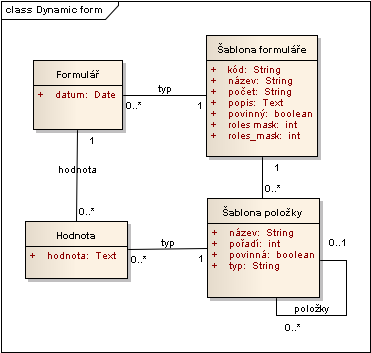
\includegraphics[scale=0.6]{figures/Dynamic_form}
\caption{Doménový model dynamických formulářů}
\label{fig:dynamicform}
\end{center}
\end{figure}

Hodnotící formuláře se generuji podle šablony formuláře získané z databáze. Šablona je reprezentovaná modelem \verb|FormTemplate|. Tato šablona obsahuje veškeré informace potřebné pro definování chování formuláře. Mezi základní vlastnosti, které definuje šablona, patří název, popis a kód. Kód šablony je velmi důležitý vlastnost, definuje skupinu kam patří formulář. Skupiny formulářů jsou rozděleny podle druhu formuláře a ty popisuji v sekci hodnocení výuky \ref{sec:formulare}. Formuláře jsou rozdělené do skupin protože se časem mohou upravovat a nemůžu si dovolit upravit již vytvořenou šablonu. Mohlo by nastat ztráta dat ve vyplněných formulářích, proto musím se musí vždy vytvořit nová šablona.  

Šablona formuláře definuje také postupné hodnocení. Pro otevření dalšího formuláře se musí splnit několik podmínek:

\begin{list}{}{}
\item Povinný formulář musí být vyplněn a také musí splnit podmínku pro minimální počet. V jiném případě není potřeba vyplnit žádný formulář.
\item Minimální počet lze definovat buď přesným počtem, nebo dynamicky podle asociace. Kde minimální počet mi definuje počet instancí v asociaci. Počet vytvořených formulářů se počítá pouze z jednoho hodnocení hospitace.
\item Hospitující i hospitovaný může vyplnit maximálně jeden formulář.
\end{list}

U dynamických formulářů jsem musel také řešit, jejich chování pro různé role v systému. Proto jsem přidal do šablony dvě bytové masky jednu pro zobrazování a druhou pro vyplňování formulářů. Používám zde princip pro identifikaci rolí viz. \ref{sec:role}.

Protože formulář Práva pro vytváření i zobrazování formulářů jsem použil stejný způsob identifikace rolí, který využívám pro role osob. Jsou obsaženy v šabloně Používám dvě masky v  jedna  identifikuje role pro tvorbu formulářů a druhá definuje role které mohou zobrazit formulář.


\begin{table}[h]
\begin{center}
\begin{tabular}{|l|c|l|}

\hline
\textbf{Typ} & \textbf{Návratová hodnota} & \textbf{Popis} \\ \hline
label &  & textový popisek \\\hline
integer & číslo & vstupní element pro čísla \\ \hline
text & text & formulář pro psaní textů \\\hline
text/file & text & formulář pro psaní textů s možností \\ & &  nahrání souboru s naskenovaným formulářem \\\hline
ranking\_table &  & tabulka pro hodnocení, může obsahovat několik \\ & & elementů typu \verb|ranking| \\\hline
column\_table & & tabulka do které se vkládají jiné elementy \\ & &  po sloupcích \\\hline
ranking & [A,B,C,D,E,F] & vstupní element pro zadávaní známkování  \\ & &   od A do F \\\hline
ranking\_scale & & tabulka s hodnotící stupnicí \\\hline
note & text & vstupní element pro napsání textové poznámky \\\hline

\end{tabular}
\caption{Seznam typů elementů}
\label{tab:elements}
\end{center}
\end{table}

Pro vygenerování obsahu formuláře používám položky formuláře reprezentované modelem \verb|EntryTemplate|. Položky formuláře definuje co se má vykreslit a kde. Umístění jednotlivých položek v dokumentu je definované ve stromové struktuře. Kde kořenem stromu je šablona formuláře a ta se postupně větví přes asociaci podpoložka. Co se má vykreslit je definované atributem typu elementu. Seznam podporovaných typů elementů a jejich vlastnosti jsou vypsány v tabulce \ref{tab:elements}. Samotné generování obsahu není složitý proces. Celý formulář se sestaví hierarchicky i s hodnotami z modelu \verb|Entry|.

Nestačí nám pouze vygenerovat formululář ale potřebujeme i uložit jeho hodnoty do databáze o to se starají modely \verb|Form| a \verb|Entry|. Model \verb|Form| složí pro identifikaci konkrétního vyplněného formuláře. Jednotlivé hodnoty z vyplněného formuláře jsou uložené v \verb|Entry|.

\subsection{Výstup} 
Výstupem této iterace byla aplikace, která již využívala pouze svoji databázi pro zdroj dat z KOSu a dynamických formulářů s nadefinovanými šablonami hodnotících formulářů.

\section{Třetí iterace}
\subsection{Zadání}
Zadáním třetí iterace bylo připravit server pro službu FELid. Dalším požadavkem bylo zprovoznění automatické zálohování databáze.

\subsection{Postup}
\subsubsection{Nasazení aplikace}
Na diagramu nasazení \ref{fig:deployment} jsou znázorněné komponenty potřebných pro rozjetí aplikace. Protože na serveru byly nainstalovány pouze webový server Apache HTTP Server a databázový systém Mysql, bylo potřeba nainstalovat platformu Ruby a framework Ruby on Rail. K instalaci Ruby jsem se rozhodl použít software RVM. Instalaci jsem provedl podle návodu pro více uživatelskou instalaci \cite{RVM}. Ten umožní nainstalovat různé platformy Ruby na jednom počítači. Mezi další přínosem je spravování gemsets\footnote{balíky knihoven mezi kterými lze přepínat pro různé aplikace}, díky nim lze zprovoznit několik aplikací zároveň na jednom počítači bez problému. Do nainstalovaného webového serveru bylo potřeba ještě přidat zásuvný modul, který umožní nasadit Rails aplikace. Modul se jmenuje Passanger (mod\_rails) a instaloval jsem ho podle návodu pro instalaci do Apache \cite{passenger}.

\subsubsection{FElid}
Pro zprovoznění služby FELid, bylo potřeba splnit několik požadavků. Tyto požadavky jsou umístěny na oficiálních stránkách služby \cite{felid_pozadavky}. Jeden z požadavků je zprovoznění programu, který zajistí komunikaci se službou FELid. Tento program se jmenuje Shibboleth a obsahuje zásuvný modul do webového serveru mod\_shib. Konfiguraci programu jsem postupoval podle návodu, který se nachází na wiki stránkách FELid \citep{felid}. Po splnění všech požadavků stačilo jen zažádat o zaregistrování aplikace.

\begin{figure}[h]
\begin{center}
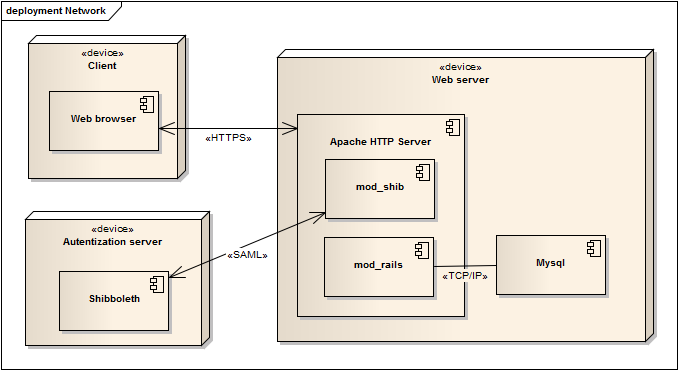
\includegraphics[width=12cm]{figures/deployment}
\caption{Diagram nasazení}
\label{fig:deployment}
\end{center}
\end{figure}

\subsubsection{Záloha databáze}
Pro automatické zálohování databáze jsem použil existující ruby aplikaci pro zálohování. Tato aplikace každý den vytvoří zálohu databáze, kterou uloží na disk. Na disku uchovává 300 záloh databáze , při překročení počtu záloh se starší zálohy nahrazují novými. Výhodou tohoto řešení je podpora různých databázových systémů a možnost ukládat zálohy na externích uložiště\footnote{pro příklad Amazon Simple Storage Service (S3)} pro uchování záloh. Záloha se spouští pravidelně každý den brzo ráno pomocí příkazu v konzoli:
\begin{verbatim}
backup perform --trigger backup
\end{verbatim} 

\subsection{Výstup} 
V této iteraci jsem se mi podařilo zprovoznit aplikaci na serveru a otestovat její funkčnost. Také jsem pracoval na programu, který jsem upravoval podle získaných připomínek od vedoucího práce.

\section{Čtvrtá iterace}
\subsection{Zadání}
Tato iterace je poslední a tím většinu zadání tvořily připomínky od vedoucího práce. Hlavními úkoly v této iteraci je vytvořit modul, který bude generovat emailové zprávy po vyplnění hodnotícího formuláře a integrovat autentizaci přes FELid. 
\subsection{Postup}
\subsubsection{Autentizace}
V této fázi vývoje byla aplikace zaregistrovaná ve FELid. Před integrování autentizace přes FELid, je potřeba otestovat aplikaci. Nejdůležitější je otestovat správnou funkčnost práv pro různé role. Pro zprovoznění autentizace přes FELid mužné jednoduše testovat aplikaci pod různými uživateli. Od zprovoznění nebudu mít totiž kontrolu nad autentizací, tu zařizuje služba FELid.

Integrace do aplikace je pak velmi jednoduchá. Stačilo jen odstranit dočasný způsob autentizace, který jsem implementoval v první iteraci. Systému FElid poskytuje informace o přihlášeném uživately prostřednictvím atributů v \verb|request.env|. Pro identifikaci přihlášeného uživatele používám atribut \verb|felid-uid| ve kterém se nachází uživatelské jméno. Autentizaci v aplikaci se stará jen jedna funkce \verb|current_user_session|.

\begin{quote}
\begin{verbatim}
def current_user_session
    return @user if defined?(@user)
    if not request.local? and not request.env["felid-uid"].nil? 
      and @user.nil? 
    then
      @user = People.find_by_username request.env["felid-uid"]
    end
    return @user
end
\end{verbatim} 
\end{quote}

\subsubsection{Emaily}
Jeden z požadavků bylo odesílání emailových zpráv po vyplnění hodnotícího formuláře. Součástí zadaná je generování emailů ze šablon. Ty půjde upravovat. Šablona se skládá z přemětu, textu zprávy a název akce. Akce v systému mohou být různých druhů, podle zadání stačilo pouze implementovat akce pro vytvoření formulářů. Při vykonání akce se vygeneruje emailová správa ze šablony emailu.

\subsubsection{Generátor obsahu emailových zpráv}
Protože je potřeba generovat do emailu proměnná data v hospitací. Tak jsem vytvořil modul \verb|EmailTemplates| pro generování emailů. Úkolem modulu je nahradit značky v textu za skutečná data. Pro vložení generovaných dat se používá zápis \verb|%značka%| do textu zprávy. 
\begin{quote}
Příklad vygenerování jednoduchého emailu se značkou pro kód předmětu.
\begin{verbatim}
text %course_code% => text A7B36ASS
\end{verbatim} 
\end{quote}

Při vývoji modulu jsem si dal za cíl vytvořit takový modul který by umožnil jednoduše nastavovat podporované značky. Největším zádrhelem v generování obsahu zprávy je v získání dat z hospitací. Vstupem do generátoru je pouze instance šablony a hodnocení hospitace. Ostatní data je potřeba získat z různých asociací.

Modul obsahuje dva pod moduly. Prvním části je modul \verb|ModelHelper|, který slouží pro rozšíření libovolného modelu v aplikaci. Rozšíření umožní pomocí metody \verb|attrs_tagged(*args)| povolit atributy, které bude možné použít pro generování emailu. 

\begin{quote}
Příklad jednoduchého nastavení modelu \verb|Person|, které umožní generátoru emailů vkládat jméno, emailovou adresu a uživatelské jméno.
\begin{verbatim}
class Person < ActiveRecord::Base
  include EmailTemplates::Tagged::ModelHelpers
    attrs_tagged :name, :email, :username
end
\end{verbatim} 
\end{quote}

Druhou částí je modul \verb|EmailBuilder|. Tento modul pomáhá si vytvořit vlastní generátor pomocí jednoduchého nastavování. Modul poskytuje metodu \verb|source(model,name,*path)| pro nastavení jednotlivých zdrojů dat. Metoda využívá k nastavení generátoru nastavení z modelu, který byl rozšířen modulem \verb|ModelHelper|, název zdroje a cestu k instancím modelu s daty. Cesta je definovaná posloupností asociací mezi modely. 

\begin{quote}
Příklad implementace jednoduchého generátoru \verb|EmailBuilder|, který dokáže vkládat do emailů informace o hospitovaném učitely. 
\begin{verbatim}
class EmailBuilder
  include Tagged::EmailBuilder
  source Person, :teacher, :evaluation, :teacher
end
\end{verbatim} 
Tento generátor bude podporovat tři značky \verb|%teacher_name%|, \verb|%teacher_email%| a \verb|%teacher_username%|. Tímto způsobem lze jednoduše nadefinovat velké množství značek.
\end{quote}

Struktura značky \ref{fig:znacka} se skládají ze dvou základních částí ze jména zdroje a jména atributu, ze kterého generátor získá data pro nahrazení značky. 
\begin{figure}[h]
\Tree [.\%teacher\_name\% [.teacher (zdroj) ]  [.name (atribut) ] ]
\caption{Struktura značky}
\label{fig:znacka}
\end{figure}

Výhodou tohoto modulu je krátký zápis a jednoduché nastavování generátoru. V aplikaci jsem celkem nadefinoval pro 9 zdrojů 32 značek.
 
\subsubsection{Odesílání emailů}
Podle zadání stačilo implementovat odesílání zpráv po akci vytvoření hodnotícího formuláře. Podle druhu hodnotícího formuláře se vygeneruje zpráva a odešle se administrátorovy hospitace, hospitujícím, hospitovaným garantovi předmětu a vedoucímu katedry. 

Z časových a technických problémů se mi nepodařilo zprovoznit emailový server pro odesílání emailů, proto dočasně používám k odesílání emailový účet hospitace-FEL-CVUT@gmail.com na Gmail.

\subsection{Výstup}
Výstupem z této iterace je finální aplikace, které splnila všechny hlavní požadavky. 